\documentclass{article}
\usepackage{amsmath}
\usepackage{graphicx}
\usepackage[utf8]{inputenc}
\usepackage{parskip}
\usepackage[symbol]{footmisc}

\renewcommand{\thefootnote}{\fnsymbol{footnote}}
\setcounter{secnumdepth}{0}

\date{}
\author{Kaan Aksoy | Feb 27, 2020}

\begin{document}

\maketitle
\section{Hurried Duelers}
\subsection{Problem}

Duels in the town of Discretion are rarely fatal.  There, 
each contestant comes at a random moment between $5$ AM and 
$6$ AM on the appointed day and leaves exactly $5$ minutes later, 
honor served, unless his opponent arrives within the time 
interval and then they fight. What fraction of duels lead to 
violence?

\subsection{Solution}

Let $X$ be the arrival time of the first contestant, and $Y$ 
that of the second. For simplicity, we will scale the duration 
between $5$ AM and $6$ AM to the value $1$, so that $\frac{1}{12}$ 
corresponds to $5$ minutes. Using this notation, the fraction of 
duels that will to violence can be stated as:

$$ P\left(|X - Y| < \frac{1}{12}\right) = 
P\left(-\frac{1}{12} < X - Y < \frac{1}{12}\right)$$

Graphing this inequality gives the following shaded region 
representing duels that lead to violence:

\begin{figure}[h]
\centering
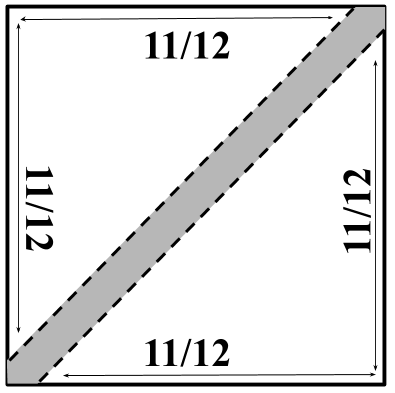
\includegraphics[width=3cm]{HurriedDuelers.png}
\caption{The shaded area represents duels that lead to violence}
\end{figure}

The relevant region is a unit square (since 
$0 \leq X \leq 1$ and $0 \leq Y \leq 1$), and $X$ 
and $Y$ are both uniformly distributed, so we can calculate 
the probability of violence as the total area of the square, 
minus the areas that do not lead to violence, which gives 
$1 - \left(\frac{11}{12}\right)^2 = \frac{23}{144} \approx \frac{1}{6}$.

\end{document}

